% !TeX program = xelatex
% 编译：在 Paper 目录运行 latexmk -xelatex main.tex（或在仓库根目录运行 latexmk -cd -xelatex Paper/main.tex）。
\documentclass{mcmthesis}

% ===== 基本信息：在此修改年份、队号、题号和论文标题 =====
\newcommand{\ContestYear}{2026}
\newcommand{\TeamNumber}{000000} % 待替换为本次参赛队号
\newcommand{\ProblemLetter}{B}
\newcommand{\PaperTitle}{Holding the Green Line: Coupled Water--Cover Dynamics, Cohort Optimization, and Compound-Hazard Resilience}
\mcmsetup{
  tstyle=\color{red}\bfseries,
  tcn=\TeamNumber, problem=\ProblemLetter,
  sheet=true, titleinsheet=true, keywordsinsheet=true,
  titlepage=false, abstract=true
}
\renewcommand{\headset}{\ContestYear\\MCM/ICM\\Summary Sheet}
\title{\PaperTitle}

\usepackage{times}
\usepackage{indentfirst}
\usepackage{needspace,tikz,subcaption,float,placeins}
\captionsetup[table]{position=top}
\renewcommand{\topfraction}{0.9}
\renewcommand{\bottomfraction}{0.85}
\renewcommand{\textfraction}{0.1}
\renewcommand{\floatpagefraction}{0.72}
\setcounter{totalnumber}{5}
\setlength{\textfloatsep}{12pt plus 2pt minus 3pt}
\usepackage{booktabs}
\usepackage{algorithm}
\usepackage[noend]{algpseudocode}
\algrenewcommand\algorithmicrequire{\textbf{Input:}}
\algrenewcommand\algorithmicensure{\textbf{Output:}}
% Wrapped algorithm lines keep their indent.
\makeatletter\newcommand{\AlgWrap}[1]{\parbox[t]{\dimexpr\linewidth-\ALG@thistlm\relax}{#1\strut}}\makeatother
\usetikzlibrary{arrows.meta,positioning,calc}
\usepackage{lastpage}
% 中英文文献库：XeLaTeX + BibTeX；正文使用 \cite{REF01} 等引用键。
\usepackage{xeCJK}
\setmainfont{texgyretermes-regular.otf}[BoldFont=texgyretermes-bold.otf,ItalicFont=texgyretermes-italic.otf,BoldItalicFont=texgyretermes-bolditalic.otf]
\setCJKmainfont{FandolSong-Regular.otf}[BoldFont=FandolSong-Bold.otf,ItalicFont=FandolKai-Regular.otf]
\setCJKsansfont{FandolHei-Regular.otf}[BoldFont=FandolHei-Bold.otf]
\setCJKmonofont{FandolFang-Regular.otf}
\usepackage[backend=bibtex,style=numeric,sorting=none,maxbibnames=3,giveninits=true]{biblatex}
\usepackage{xurl}
\addbibresource{bibliography/references.bib}
% 有 DOI 时不重复输出同一文献的网址。
\AtEveryBibitem{%
  \iffieldundef{doi}{}{\clearfield{url}}%
  \clearfield{urlyear}\clearfield{urlmonth}\clearfield{urlday}%
}
\graphicspath{{Figure/}}
\geometry{headheight=14pt}
\setlength{\emergencystretch}{1.2em}
\hypersetup{hidelinks,pdfauthor={},pdftitle={MCM/ICM Paper}}

% Shared colour palette for inline TikZ schematics and executive brief
% Shared colours for the TikZ schematics; same roles and hex values as
% Code/figures_matlab/paper_style.m (mycolor.space, base #1E5F74).
%   water (P, I, M, W-bar)  teal   | vegetation (V, r, d)  green
%   wind and sand (E, S)    brown  | highlight             orange
%   limits and caps         red dashed
\definecolor{pWater}{HTML}{1E5F74}
\definecolor{pWaterMid}{HTML}{659FB6}
\definecolor{pWaterLight}{HTML}{DCEBF1}
\definecolor{pTeal}{HTML}{00828C}
\definecolor{pVeg}{HTML}{2B633C}
\definecolor{pVegMid}{HTML}{4AC087}
\definecolor{pVegLight}{HTML}{E3F3E8}
\definecolor{pSand}{HTML}{8F7159}
\definecolor{pSandLight}{HTML}{FFEACE}
\definecolor{pAccent}{HTML}{F49431}
\definecolor{pPV}{HTML}{D47216}
\definecolor{pPVLight}{HTML}{FDF1E3}
\definecolor{pPlum}{HTML}{7A437F}
\definecolor{pPlumLight}{HTML}{F2EBF3}
\definecolor{pLimit}{HTML}{D03B3B}
\definecolor{pInk}{HTML}{1F2B33}
\definecolor{pAxis}{HTML}{344A53}
\definecolor{pGrey}{HTML}{97AFB9}
\definecolor{pGreyDark}{HTML}{647B84}
\definecolor{pGrid}{HTML}{E6EBED}


% 保留旧论文的符号表、公式分组和交替灰底表格工具。
\newcommand{\shade}{\rowcolor{gray!22}}
\newcommand{\modelvars}[1]{%
  \par\begingroup\small
  \setlength{\tabcolsep}{4pt}\renewcommand{\arraystretch}{1.10}
  \noindent\begin{tabularx}{\linewidth}{@{}>{\raggedright\arraybackslash}p{0.29\linewidth} >{\raggedright\arraybackslash}X@{}}
  \toprule\textbf{Symbol} & \textbf{Meaning} \\\midrule
  #1
  \bottomrule\end{tabularx}\par\endgroup
}
\newenvironment{modeleq}
  {\par\addvspace{0.4\baselineskip}\noindent\begin{minipage}{\linewidth}\setlength{\abovedisplayskip}{6pt}\setlength{\belowdisplayskip}{6pt}}
  {\end{minipage}\par\addvspace{0.4\baselineskip}}

% Bold run-in paragraph headings (template prints them plain).
\makeatletter
\renewcommand\paragraph{\@startsection{paragraph}{4}{\z@}{1.2ex \@plus .5ex}{-1em}{\normalfont\normalsize\bfseries}}
\makeatother

% Float pages start at the top instead of being vertically centred.
\makeatletter\setlength{\@fptop}{0pt}\makeatother

\begin{document}

% ===== 第一页：Summary Sheet（摘要不编入正文章节编号） =====
\begin{abstract}
Spatial closure of the Taklamakan Desert's protective belt does not ensure persistence over decades; holding it requires coordinating seasonal water scarcity, finite budgets and labour, and compound hazards. We build a state-consistent modelling chain in which vegetation cover and root-zone soil moisture pass sequentially from biophysical calibration (\textbf{Model~1}), through multi-year scheduling (\textbf{Model~2}), to stochastic stress testing (\textbf{Model~3}) and operational policy.

\textbf{Coupled eco-hydrology (Model~1).} Model~1 couples an inner \emph{daily} soil-water bucket to an outer \emph{annual} logistic cover equation via the annual water-satisfaction ratio, with day-to-day wind acting solely through Penman--Monteith evaporative demand. Without irrigation, long-run cover settles at $1.8\%$; irrigation lifts the plateau to $17.9\%$ at $300$\,mm/yr and $24.1\%$ at $600$\,mm/yr with sharply diminishing returns (capping at $30.6\%$), while $20\%$ stronger wind costs $0.7$ percentage points of cover and raises sand exposure.

\textbf{Cohort optimisation and PV cross-subsidy (Model~2).} Pre-simulating dated planting--irrigation \emph{cohorts} in Model~1 casts the 15-year allocation of planting, water, labour, and photovoltaics (PV) as an exact mixed-integer linear $\varepsilon$-constraint problem. At the $60\%$ ecological target, the optimal plan plants $3$\,square kilometers in years 1--2, ramps water with stand age, and installs $9.5$\,MW of PV across years 1--4 (CNY~$44.3$\,million upfront capital). Annual PV revenue (CNY~$4.1\text{--}4.3$\,million) exceeds upkeep and water costs (CNY~$1.8\text{--}2.0$\,million), cutting net present cost by $9\%$ to CNY~$25.35$\,million while exposing May demand ($95\%$ of monthly canal capacity) as the tightest seasonal water constraint.

\textbf{Compound-hazard resilience (Model~3).} Inheriting Model~2's year-15 cohorts directly, Model~3 evaluates 50-year persistence under climate drift, drought switches, and compound-Poisson storms with monthly canal rationing, cross-checked against a 2-D discretised Markov chain. The 50-year restricted mean time to the first belt warning is $7.1$\,years ($16.1$\,years on the $600$\,mm/yr core strip). By year~50, about $99$\,ha have recovered above the warning threshold and about $200$\,ha remain below it. The belt retains $65.5\%$ of the cumulative ecological benefit under climate drift alone. Storm severity and monthly limits on drought-year water delivery govern resilience.

\textbf{Operational synthesis.} Translating these findings into a phased plan aligns spring canal checks, age-staged upkeep, ring-fenced PV financing, and post-hazard repair for holding the belt.

\begin{keywords}
Taklamakan protective belt; Two-clock eco-hydrology; Cohort MILP; Agrivoltaic cross-subsidy; Compound-Poisson resilience; Discretised 2-D substochastic Markov chain
\end{keywords}
\end{abstract}
\hypersetup{pageanchor=false}
\maketitle
\hypersetup{pageanchor=true}

% ===== 第二页起：目录及正文 =====
\pagestyle{main}
% Keep the complete contents on one page without changing body typography.
\begingroup
\small
\setlength{\parskip}{0pt}
\tableofcontents
\endgroup
\clearpage

\section{Introduction}
\subsection{Problem background}
Spanning roughly $337{,}600\,\text{km}^2$, the Taklamakan Desert is China's largest shifting-sand desert and one of the most hyper-arid basins on Earth. In November 2024, China completed spatial closure of a $3{,}046$\,km ``Green Sand-Blocking Protective Belt'' encircling the desert margin \cite{REF12}. Yet sand control is an ongoing management task rather than a one-off engineering milestone: \emph{closing} the perimeter on a map does not guarantee \emph{holding} it over decades. Sustaining the belt requires balancing a coupled, non-stationary system shaped by scarce seasonal water, finite multi-year budgets, construction and maintenance labour, and stochastic natural hazards \cite{REF06} (\textbf{Table~\ref{tab:protection-factors}}).

\begin{table}[htbp]
  \centering
  \caption{Key factors and quantities in protective-belt management.}
  \label{tab:protection-factors}
  \begingroup\small
  \renewcommand{\arraystretch}{1.18}
  \begin{tabularx}{\linewidth}{@{}>{\raggedright\arraybackslash}p{0.17\linewidth}
    >{\raggedright\arraybackslash}p{0.37\linewidth}
    >{\raggedright\arraybackslash}X@{}}
    \toprule
    \textbf{Factor} & \textbf{Representative quantities} & \textbf{Role in belt protection} \\
    \midrule
    Water supply & Ecological replenishment volume ($\text{m}^3$/yr); monthly irrigation timing
      & Sustains root-zone soil moisture and vegetation growth under extreme evaporative demand. \\
    Funding & Total budget (CNY); allocation shares in construction, O\&M, and supporting PV
      & Sets newly treated belt scale, photovoltaic revenue capacity, and ongoing maintenance. \\
    Labour & Annual workforce input (person-days/yr); construction vs.\ upkeep split
      & Supports shrub planting, seasonal irrigation, panel installation, and stand upkeep. \\
    Disaster shocks & Drought probability; storm frequency ($\text{yr}^{-1}$) and fractional cover loss
      & Causes canopy defoliation/burial, shrinks canal supply, and tests biological recovery. \\
    \bottomrule
  \end{tabularx}
  \endgroup
\end{table}

\subsection{Problem restatement}
\begin{enumerate}
  \item Establish a coupled dynamic model (Task 1).
  Use public meteorological and remote-sensing observations to quantify \textbf{vegetation coverage},
  \textbf{effective root-zone soil moisture}, and their \textbf{interactions with wind and sand}.

  \item Optimise construction and resource allocation (Task 2).
  Make an explicit trade-off between ecological benefits and economic costs over a 15-year horizon under a fixed budget and resource caps. Optimise \textbf{annual newly treated area}, \textbf{age-scheduled water replenishment}, \textbf{investment allocation ratios} across construction, O\&M, and revenue-generating photovoltaics (PV), and \textbf{labour input}; test \textbf{investment sensitivity} and derive an \textbf{actionable process criterion}.

  \item Assess resilience and long-term benefits (Task 3).
  Embed \textbf{stochastic compound disasters} (sandstorms, extreme droughts, wind erosion, and sand burial) and \textbf{climate-driven baseline drift} into the post-construction belt. Quantify \textbf{resistance and post-shock recovery} alongside \textbf{long-term ecological trajectories}.

  \item Deliver an actionable policy and public brief (Task 4).
\end{enumerate}

\subsection{Our work}
\begin{figure}[H]\centering
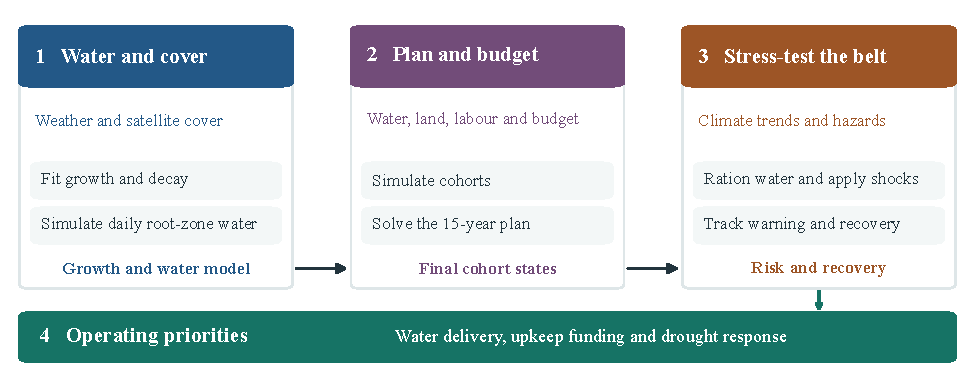
\includegraphics[width=\linewidth]{../Figures/Paper2026_Mechanisms/workflow_cards.pdf}
\caption{From model calibration to an operating plan.}\label{fig:framework}
\end{figure}

\subsection{Assumptions and Justifications}
\begingroup
\setlength{\topsep}{0pt}
\setlength{\partopsep}{0pt}
\setlength{\parsep}{0pt}
\setlength{\itemsep}{4pt}
\begin{enumerate}
  \item \textbf{Assumption: The reference section is locally uniform.} We use the Yutian and Minfeng satellite records to represent average conditions along the section. Within-section variation is unresolved.
  \newline \textbf{Justification:} Public data support section-scale analysis, not fine-scale heterogeneity.

  \item \textbf{Assumption: Soil water evolves daily and cover annually.} One root-zone store carries water between years; salinity feedback is omitted.
  \newline \textbf{Justification:} The two timescales capture dry spells and slow growth; omitting salinity may overstate long-term water benefits \cite{REF01,REF04}.

  \item \textbf{Assumption: Construction uses discrete lots and constant real unit costs.} New PV panels begin generating revenue in the year after installation.
  \newline \textbf{Justification:} Lots reflect field contracting; real prices make yearly cash flows comparable.

  \item \textbf{Assumption: Disaster risks follow declared stress-test scenarios.} During shortages, PV washing is supplied first and remaining canal water is shared proportionally among stands.
  \newline \textbf{Justification:} Without a local damage catalogue, explicit scenarios and allocation rules support conditional stress tests rather than calibrated forecasts.
\end{enumerate}
\endgroup

\section{Model Preparations}\label{sec:data}
\subsection{Study area and station categories}
The shelterbelt lies between the Taklamakan's river-fed oases and its dune fields~\cite{REF06}. Seven oasis-margin sites (YT, MF, QM, RQ, KEL, YL and ALE) calibrate Model~1. Yutian and Minfeng define the 128\,km reference transect. XT represents the saline-drip corridor along the Desert Highway~\cite{REF01}, and TZ provides the desert-interior control. Figure~\ref{fig:data-stations} uses Esri World Imagery and marks one standard deviation of summer cover across years.

\begin{figure}[H]
  \centering
  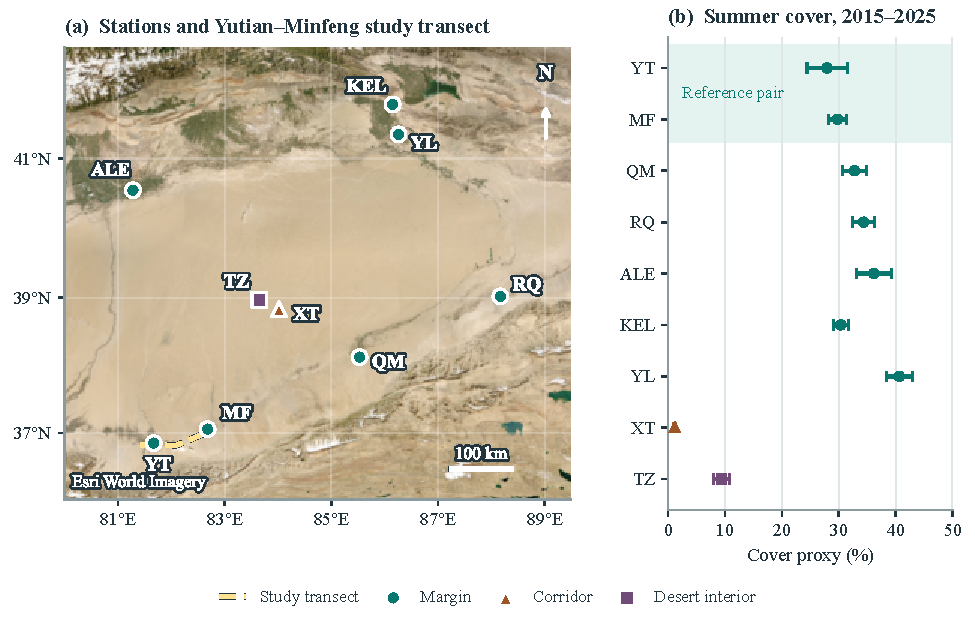
\includegraphics[width=\linewidth]{../Figures/Paper2026/02_study_area.pdf}
  \caption{Study sites and summer vegetation cover, 2015--2025.}
  \label{fig:data-stations}
\end{figure}

\subsection{Data sources and preprocessing}
The panel contains 1,188 records (nine sites over 132 months, 2015--2025) and 395 valid summer cover values out of 396. Each summer mean uses at least two valid months. NASA POWER supplies temperature, rainfall and wind~\cite{REF17}. Monthly precipitation totals equal the reported daily rate times days per month. XT and TZ share a MERRA-2 grid cell, leaving eight independent weather series. Open-Meteo provides reference evapotranspiration~\cite{REF19,EN10}. We omit SoilGrids inputs after only 62 of 81 queries returned profiles~\cite{EN09}.

We apply the wind-transport proxy to each day's peak wind above $5$\,m/s before averaging, then divide by the site mean for 2015--2022. This index $E$ tracks relative exposure. Model~1 uses wind speed in evaporative demand, and Model~3 represents acute cover loss.

For MOD13Q1 we keep pixels with reliability flag at most 1 within each $9\times9$ window~\cite{REF18}. Composites need at least 50\% of their pixels (75\% in the sensitivity check). We take the monthly maximum and convert NDVI to a cover proxy via
\begin{equation}
  V = \operatorname{clip}\!\left(\frac{\mathrm{NDVI}-0.05}{0.85-0.05},\,0,\,1\right)\times100\%.
\end{equation}

\section{Notations}
\modelvars{%
  $t,\ m,\ j$ & Year index, month ($m=1,\dots,12$), and day ($j=1,\dots,365$) or cohort index in Model~3 \\
  \shade $(s,\,p)$ & Cohort planted in year $s$ under lifetime irrigation policy $p\in\mathcal P$ \\
  $V_t,\ M_j$ & Growing-season vegetation cover proxy (\%) and root-zone soil water (mm) \\
  \shade $D_j,\ T_{a,j},\ \overline W_t$ & Daily water demand, actual transpiration (mm/d), and annual demand-met ratio \\
  $E_t,\ S_t$ & Relative wind-transport index and sand-exposure index $E_t(1-V_t/K)$ \\
  \shade $n_{s,p},\ z_s$ & Integer counts of shelterbelt parcels ($\Delta_A$) and PV units ($\Delta_P$) \\
  $a_t,\ A_t$ & Newly treated belt area (flow) and active belt area in service (stock, ha) \\
  \shade $y_t,\ P_t^{\mathrm{inst}},\ P_t^{\mathrm{op}}$ & Newly built, cumulative installed, and operating PV capacity (kW or MW) \\
  $Q_t,\ Q_{t,m};\ L_t$ & Annual and monthly gross water withdrawal ($\text{m}^3$); annual labour (p-d) \\
  \shade $D_t,\ (f_t^b,f_t^o,f_t^p),\ R_t$ & Gross spending (CNY), allocation ratios (build / O\&M / PV), and PV income (Model~2) \\
  $H,\ N$ & Cumulative ecological cover integral ($\text{effective ha}\cdot\text{yr}$) and net present cost (CNY) \\
  \shade $D_t^{\mathrm{dr}},\ N_t,\ R_t$ & Drought state, Poisson storm count, and multiplicative cover retention (Model~3) \\
  $\tau_j,\ \tau_{\mathrm{proj}},\ \mathrm{RMST}$ & Cohort/project first-crossing year below $\rho K$ and 50-yr restricted mean survival time (yr) \\
}

\section{Model of Desertification Control and Construction}
% Model 1 couples daily root-zone water with annual cover.
\subsection{Coupled Vegetation--Water--Sand Dynamics}\label{sec:model1}
\subsubsection[Daily Water Balance and Annual Vegetation Growth]{Model construction}
\paragraph{Two states on two timescales.} Annual cover $V_t$ sets daily transpiration demand $D_j$. We divide the monthly forcing and assigned irrigation evenly among the days of each month and update plant-available root-zone water $M_j$ in mm at each step. At year end, the fraction of demand met drives the cover update, and the remaining water carries into the next year (Figure~\ref{fig:m1-clocks}).

\begin{figure}[!htb]
  \centering
  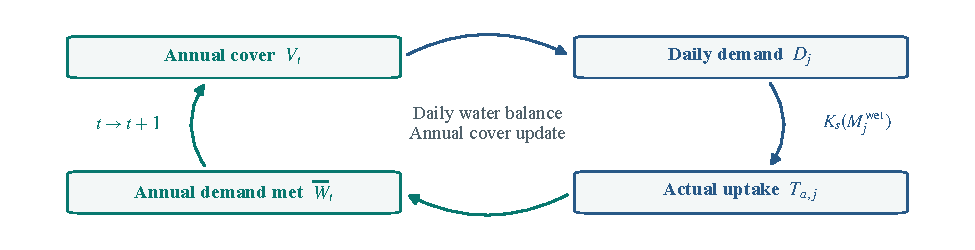
\includegraphics[width=\linewidth]{../Figures/Paper2026_Mechanisms/m1_water_feedback.pdf}
  \caption{Daily water uptake and annual cover feedback.}
  \label{fig:m1-clocks}
\end{figure}

\paragraph{Cover equation: growth and decay.}
\begin{equation}\label{eq:m1-veg}
V_{t+1}=V_t+\underbrace{rV_t\Big(1-\frac{V_t}{K}\Big)\overline W_t}_{\text{growth, limited by water}}
-\underbrace{dV_t}_{\text{natural decay}}
\end{equation}
\emph{Growth} is logistic, stops at the local ceiling $K$, and is scaled by the water-satisfaction ratio $\overline W_t\in[0,1]$ (Eq.~\eqref{eq:m1-wbar}). \emph{Decay} removes a fixed share $d$ of cover each year. There is no separate wind term; wind enters through the water demand below. Since $V=0$ stays at $0$, every scenario starts from a planted cover.

\paragraph{Root-zone water balance.} Add the effective fractions of rain and irrigation to the starting store $M_j$ and drain water above capacity $C$ (Figure~\ref{fig:m1-bucket}). The resulting available store is $M_j^{\mathrm{wet}}$:
\begin{equation}\label{eq:m1-bucket}
M_j^{\mathrm{wet}}=\min\!\big(C,M_j+\alpha_PP_j+\eta_wI_j\big),\qquad
T_{a,j}=\min\!\big(M_j^{\mathrm{wet}},K_sD_j\big),\qquad
M_{j+1}=M_j^{\mathrm{wet}}-T_{a,j}.
\end{equation}
The daily demand and the stress coefficient are
\begin{equation}\label{eq:m1-demand}
D_j=c\,\min\!\Big(1,\frac{2V_t}{V_{\mathrm{full}}}\Big)\,f(T_j)\,\mathrm{ET}_{0,j},\qquad
K_s=\min\Big\{1,\ \frac{M_j^{\mathrm{wet}}}{(1-p)C}\Big\}.
\end{equation}
The transpiration coefficient $c$ scales reference evapotranspiration $\mathrm{ET}_0$ to stand demand. Demand rises with cover up to $V_{\mathrm{full}}/2$. The seasonal factor $f(T)$ is zero at or below $5\,^\circ\mathrm{C}$ and reaches one at $25\,^\circ\mathrm{C}$. The FAO-56 coefficient $K_s$ limits uptake below the baseline available-water threshold of $37.5$\,mm~\cite{REF11}. Figure~\ref{fig:m1-stress} shows both multipliers, with 2015--2022 monthly mean temperatures from Yutian and Minfeng marked on $f(T)$.

\begin{figure}[!htbp]
  \centering
  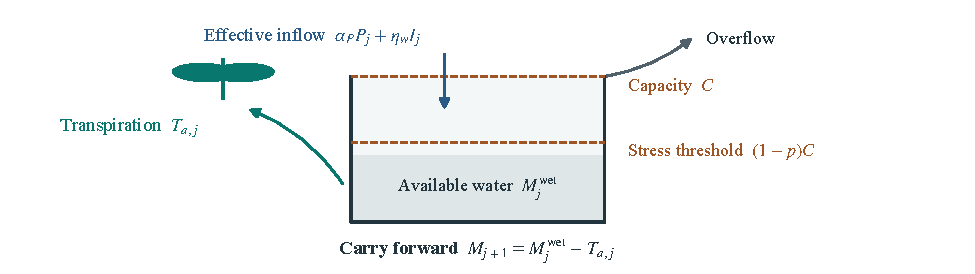
\includegraphics[width=\linewidth]{../Figures/Paper2026_Mechanisms/m1_root_zone.pdf}
  \caption{One daily step of the root-zone water balance.}
  \label{fig:m1-bucket}
\end{figure}

\begin{figure}[!htbp]
  \centering
  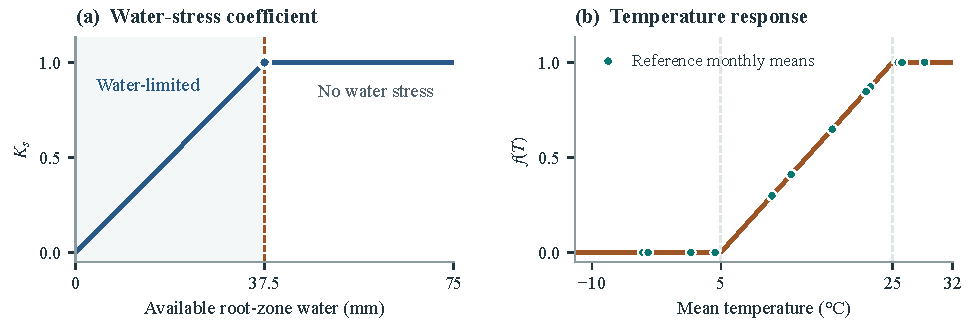
\includegraphics[width=\linewidth]{../Figures/Paper2026_Polished/fig05_stress_switches.pdf}
  \caption{Water-stress and temperature response functions.}
  \label{fig:m1-stress}
\end{figure}

\paragraph{The link between the two clocks.} The daily bucket and the yearly cover update are coupled through one number, the water-satisfaction ratio
\begin{equation}\label{eq:m1-wbar}
\overline W_t=\frac{\sum_{j\in t}T_{a,j}}{\sum_{j\in t}D_j},
\end{equation}
the share of plant water demand actually met in year $t$. No water stress ($\overline W_t=1$, as in oases) yields full growth rate $r$; intermediate values scale growth proportionally ($\overline W_t=0.4$ reduces growth to $0.4\,r$); and $\overline W_t=0$ halts growth, leaving only decay.

\paragraph{Wind: water demand and disaster damage.} We distinguish two pathways. In Model~1, day-to-day wind affects growth through evaporative demand. The reference evapotranspiration $\mathrm{ET}_0$ in Eq.~\eqref{eq:m1-demand} follows FAO-56 Penman--Monteith \cite{REF11},
\begin{equation}\label{eq:m1-pm}
\mathrm{ET}_0=\frac{0.408\,\Delta\,(R_n-G)+\gamma\,\dfrac{900}{T+273}\,u_2\,(e_s-e_a)}{\Delta+\gamma\,(1+0.34\,u_2)},
\end{equation}
where $u_2$ is the wind speed at 2\,m, $R_n-G$ the available energy, $e_s-e_a$ the dryness of the air, and $\Delta$, $\gamma$ thermodynamic coefficients. At baseline, the aerodynamic term accounts for 61\% of annual reference $\mathrm{ET}_0$. Wind speed enters both the numerator and the denominator, so this share differs from the response to changing wind speed. A windier climate therefore raises the demand $D_j$, lowers $\overline W_t$ and slows growth.

In Model~1, the index $S_t=E_t(1-V_t/K)$ tracks relative sand exposure: higher cover leaves less surface exposed. We use $S_t$ only as a diagnostic because the annual observations cannot isolate direct wind damage to vegetation. Model~3 treats direct cover loss from severe storms separately.

The growing-season weighting reduces annual reference demand from 1,686 to 1,191\,mm/yr (Figure~\ref{fig:m1-sens}a). At long-run quotas of 300 and 600\,mm/yr, year-end storage remains below the stress threshold.

\subsubsection[Least-Squares Calibration and Long-Run Simulation]{Solution approach}
We fit growth and decay from data, step the coupled system through a year, and repeat the year to reach a long-run state or a scenario path.

\paragraph{Step 1: calibration by least squares.} At the seven oasis stations water is ample ($\overline W\approx1$), so we set $\overline W=1$ there; growth and decay can then be estimated from cover alone. Fixing $K$ from each station's own record and writing $x=V/K$, Eq.~\eqref{eq:m1-veg} becomes
\begin{equation}\label{eq:m1-reg}
\underbrace{x_{s,t+1}-x_{s,t}}_{y_{s,t}:\ \text{observed change}}=r\,\underbrace{x_{s,t}(1-x_{s,t})}_{z_{1,s,t}:\ \text{growth signal}}-d\,\underbrace{x_{s,t}}_{z_{2,s,t}:\ \text{decay signal}}+\varepsilon_{s,t},
\end{equation}
where $s$ indexes stations and $\varepsilon_{s,t}$ is the one-step error. The model is linear in the unknowns $(r,d)$, so we estimate them by ordinary least squares over the set $\mathcal T$ of training pairs (target year $\le2022$, all seven stations pooled):
\begin{equation}\label{eq:m1-ls}
(\hat r,\hat d)=\arg\min_{r,d}\ \sum_{(s,t)\in\mathcal T}\big(y_{s,t}-(r\,z_{1,s,t}-d\,z_{2,s,t})\big)^2 .
\end{equation}
We solve Eq.~\eqref{eq:m1-ls} with design matrix $\bm Z=[\,\bm z_1,-\bm z_2\,]$. To estimate uncertainty, we resample whole stations with replacement, keeping each station's time series intact, and refit $(r,d)$ for each bootstrap sample.

\paragraph{Steps 2--3: one model year, then repeat.} Algorithm~\ref{alg:m1} shows the core loop. Repeating it under a typical climate year until $V$ and $M$ stop changing gives the long-run state for a given irrigation level. Because $\overline W$ depends on $V$, this fixed point is found numerically; we start from both a low and a high cover and accept the result only when both starts agree.

\begin{algorithm}[H]
\caption{One model year: the water store drives cover}\label{alg:m1}
\begin{algorithmic}[1]
\Require cover $V_t$, store $M$, irrigation $I_t$, monthly rain, ET$_0$ and temperature
\Ensure $V_{t+1}$, year-end store $M$, $\overline W_t$
\State Set daily demand $D_j$ from $V_t$ and the season \Comment{cover held fixed}
\For{each day $j$ of the year}
  \State $M\gets M+\alpha_PP_j+\eta_wI_j$;\quad spill anything above $C$ \Comment{inflow subtract overflow}
  \State $T_{a,j}\gets\min\big(M,K_s(M)D_j\big)$;\quad $M\gets M-T_{a,j}$ \Comment{water index is stressed when $M$ is low}
\EndFor
\State $\overline W_t\gets\sum_jT_{a,j}/\sum_jD_j$ \Comment{Eq.~\eqref{eq:m1-wbar}}
\State $V_{t+1}\gets$ Eq.~\eqref{eq:m1-veg};\quad carry $M$ into next year
\end{algorithmic}
\end{algorithm}

\begin{table}[H]
\centering\small
\caption{Parameter values for Model 1.}
\label{tab:m1-par}
\renewcommand{\arraystretch}{1.1}
\begin{tabularx}{\linewidth}{@{}l X r c l@{}}
\toprule
Symbol & Meaning & Value & Range tested & Unit \\
\midrule
\multicolumn{5}{@{}l}{\textit{Fitted by least squares (Eq.~\eqref{eq:m1-ls})}}\\
$r$ & intrinsic growth rate & 0.547 & 0.335--1.168$^{\dagger}$ & yr$^{-1}$ \\
$d$ & natural decay rate & 0.107 & 0.077--0.202$^{\dagger}$ & yr$^{-1}$ \\
\midrule
\multicolumn{5}{@{}l}{\textit{Set from data by a fixed rule}}\\
$K$ & cover ceiling ($1.15\times$ 95th percentile of training cover) & 38.08 & -- & \% \\
$V_{\mathrm{full}}$ & oasis end-member used to scale demand & 66.59 & 64.85--69.40 & \% \\
\midrule
\multicolumn{5}{@{}l}{\textit{Assumed}}\\
$C$ & root-zone storage capacity & 75 & 30--150 & mm \\
$p$ & stress-free share of storage (FAO-56 \cite{REF11}) & 0.5 & 0.3--0.7 & -- \\
$c$ & transpiration coefficient & 1.0 & 0.7--1.2 & -- \\
$\eta_w$ & share of irrigation reaching the roots (FAO-56 \cite{REF11}) & 0.75 & 0.65--0.85 & -- \\
$\alpha_P$ & share of rain reaching the roots (FAO-56 \cite{REF11}) & 0.25 & 0--1 & -- \\
$u_T$ & wind threshold in the index $E_t$ & 5 & -- & m/s \\
$V_0$ & initial cover of a new stand & 2 & -- & \% \\
$M_0$ & initial store of a new stand & 37.5 & -- & mm \\
\bottomrule
\end{tabularx}
\end{table}

\subsubsection[Vegetation Response to Irrigation and Wind]{Results}

\paragraph{Model reliability.} Across the 21 held-out site-years, one-step RMSE in $V/K$ is 0.0635 for Model~1 and 0.0536 for persistence. The model improves on persistence at the two reference sites, Yutian and Minfeng, but has larger errors at the other five (Figure~\ref{fig:m1-obs}a). A free run from 2022 illustrates the limitation at Ruoqiang: predicted cover is 33.0\% in 2025 against 38.4\% observed (panel d). We therefore use Model~1 to compare irrigation strategies.

\begin{figure}[!htbp]
  \centering
  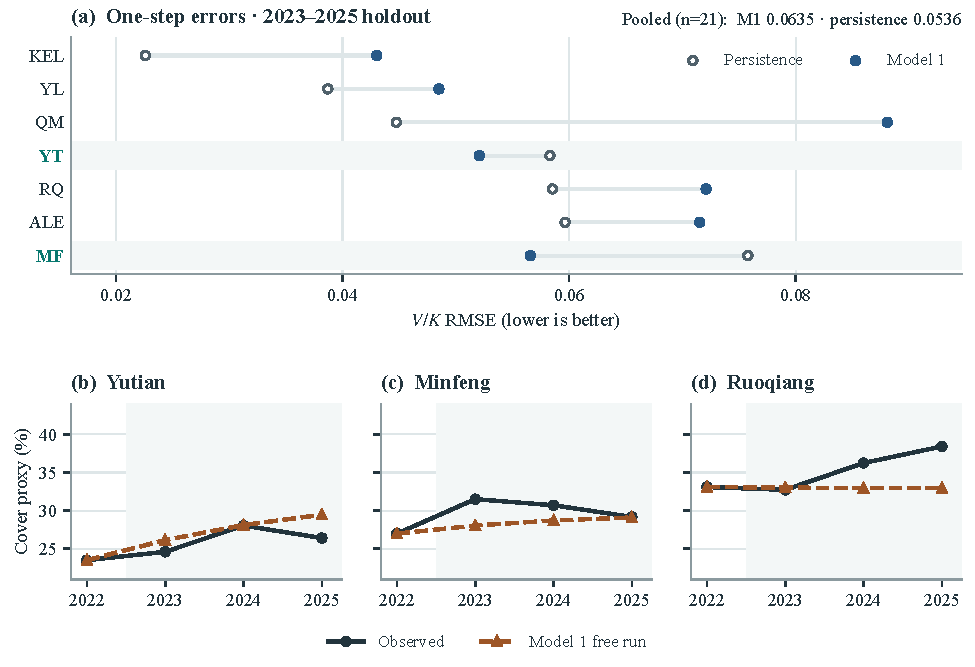
\includegraphics[width=\linewidth]{../Figures/Paper2026_Polished/fig06_holdout.pdf}
  \caption{Holdout errors and cover trajectories.}
  \label{fig:m1-obs}
\end{figure}

\paragraph{Evolution of the state variables.} From a planted cover of 2\%, cover and soil water pass through three phases (Figure~\ref{fig:m1-curve}b,d):
\begin{enumerate}\setlength{\itemsep}{1pt}\setlength{\parsep}{0pt}
  \item \textbf{Establishment: growth, not water, limits cover.} Young plants use little water. All plotted quotas of 300\,mm/yr or more meet demand ($\overline W=1$) through 2030 and reach 9.9\% cover at year-end. Extra irrigation does not increase cover in this phase.
  \item \textbf{Transition: cover drains the store.} Demand rises with cover until it exceeds supply. The store then drops from capacity within about two years and settles slowly (to about 13.5\,mm at 300\,mm/yr), and $\overline W$ falls below one. This is the feedback at work: more cover means less water per plant, which slows growth.
  \item \textbf{Plateau (after 15--25 years): both settle.} By 2050, cover and year-end storage are near their plateaus: 17.9\% and 13.5\,mm at 300\,mm/yr, and 24.1\% and 19.3\,mm at 600\,mm/yr.
\end{enumerate}
Trajectories repeat 2015--2022 weather. In the stop scenario, irrigation is 600\,mm/yr through 2035. In the first year after irrigation stops, year-end storage falls from 22.8 to 0.81\,mm and $\overline W$ falls to 0.045. Cover falls from 21.5\% to 12.7\% after five years and to 5.1\% after fifteen years.

\paragraph{Controlling factors: water supply.} Water supply is the main control. Without irrigation, annual rainfall of 52\,mm against roughly 1,700\,mm of reference evaporative demand sustains only 1.8\% long-run cover in the model.

The first 100\,mm/yr adds 7.7 percentage points of long-run cover, while increasing the quota from 500 to 600\,mm/yr adds only 1.6 points. At 300\,mm/yr only 37\% of demand is met. Beyond about 1,500\,mm/yr, additional water overflows and the cover proxy levels off at 30.6\% (Figure~\ref{fig:m1-curve}a,c).

\begin{figure}[!htbp]
  \centering
  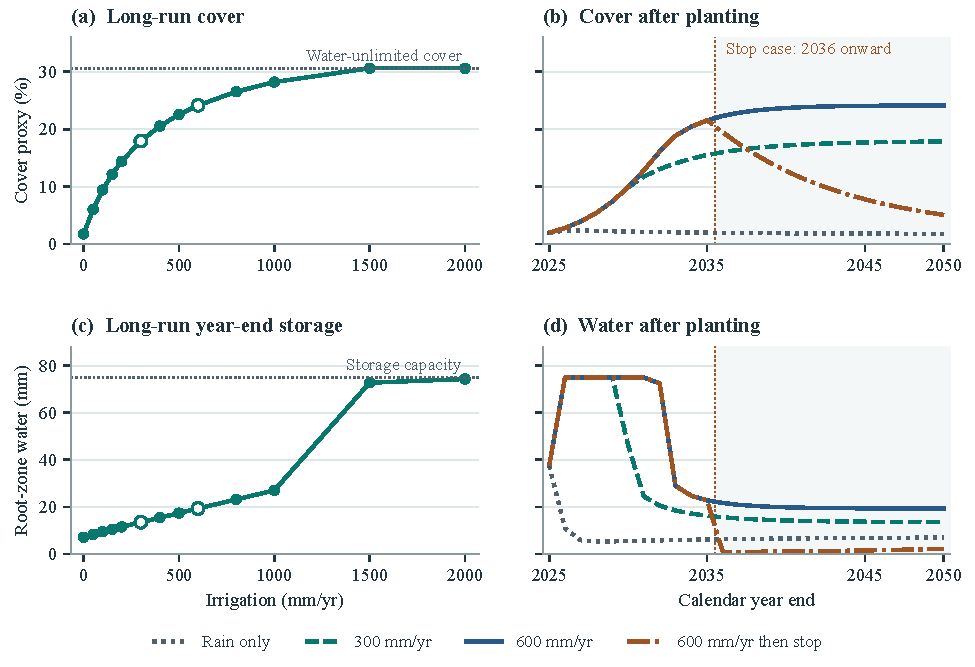
\includegraphics[width=\linewidth]{../Figures/Paper2026_Polished/fig07_irrigation_response.pdf}
  \caption{Cover and root-zone storage under alternative irrigation schedules.}
  \label{fig:m1-curve}
\end{figure}

\paragraph{Controlling factors: demand, delivery and wind.} With water supply fixed, we varied the other factors one at a time (Figure~\ref{fig:m1-sens}). They fall into three groups:
\begin{enumerate}\setlength{\topsep}{1pt}\setlength{\itemsep}{0pt}\setlength{\parsep}{0pt}
  \item \textbf{Factors that shift long-run cover by 1--3 points:} the transpiration coefficient $c$ ($-1.7$ to $+3.4$ points at 300\,mm/yr), irrigation efficiency ($\pm1.2$) and the effective rain fraction ($-0.5$ to $+1.4$). All three act through $\overline W$, the supply-to-demand ratio.
  \item \textbf{Factors that change soil water but not long-run cover:} storage capacity and the stress threshold. Without overflow, all inflow is eventually transpired, so $\overline W$ depends only on inflow and demand; these factors change only the storage level and its timing.
  \item \textbf{Wind, through evaporative demand.} Scaling wind speed in Eq.~\eqref{eq:m1-pm} by $+20\%$ raises season-adjusted reference demand by 7.7\% and lowers long-run cover at 300\,mm/yr from 17.9\% to 17.2\%; $-20\%$ raises it to 18.8\% (Figure~\ref{fig:m1-sens}b). Less cover leaves more sand exposed: $S$ moves from 0.53 to 0.55.
\end{enumerate}
\begin{figure}[!htbp]
  \centering
  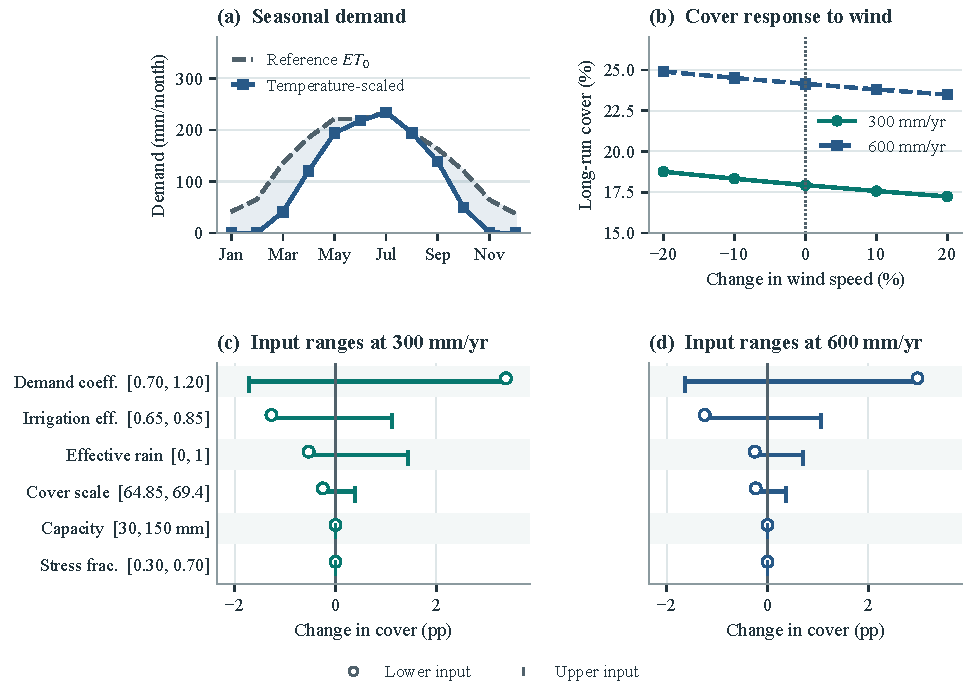
\includegraphics[width=\linewidth]{../Figures/Paper2026_Polished/fig08_drivers.pdf}
  \caption{Demand, wind response and drivers of long-run cover.}
  \label{fig:m1-sens}
\end{figure}

\paragraph{Summary.} Cover and soil water rise together, settle at a level set by the water supply, and decline once water stops. Water supply is the main control, with sharply diminishing returns. Wind acts through the water demand: 20\% more wind costs about 0.7 points of cover, and cover in turn decides how much sand stays exposed.


% Model 2 sketch: concise logic chain, 4 core formulas, visual restriction chart,
% and results aligned with Task 2's three questions in Problem B.
\subsection{Optimal Investment, Scheduling and Resource Allocation}\label{sec:model2}
Task~2 turns Model~1 into a 15-year dynamic decision problem: how much belt to plant each year, how to schedule ecological water and labour, and how to split funds among construction, O\&M and photovoltaics (PV) under a fixed budget.

Planting and PV installation create dated cohorts. The optimiser carries each cohort's cover and stored water forward and charges it for water, labour and maintenance. PV competes for the construction budget and subsequently earns revenue (Figure~\ref{fig:m2-struct}).

\begin{figure}[!htb]
  \centering
  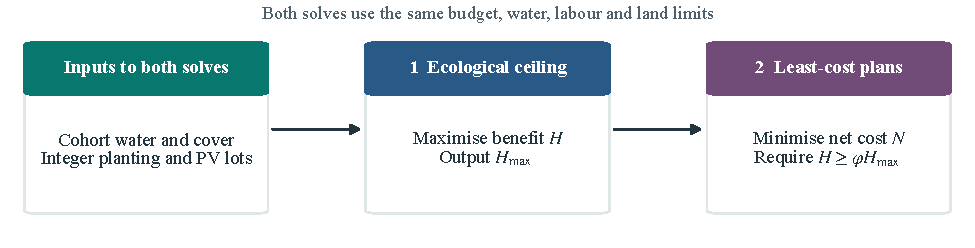
\includegraphics[width=\linewidth]{../Figures/Paper2026_Polished/fig09_two_stage_optimisation.pdf}
  \caption{Two-stage optimisation of the planting and PV plan.}
  \label{fig:m2-struct}
\end{figure}

\subsubsection[Cohort Irrigation, PV Revenue, and Resource Limits]{Model construction}
\paragraph{Cohort formulation and ecological benefit.} Tracking only total area $A_t$ cannot distinguish a newly planted shrub ($V_0=2\%$, low water demand) from an older stand ($>12\%$ cover, high summer demand). Instead, we bind each planting year $s\in\{1,\dots,T\}$ and lifetime watering recipe $p\in\mathcal P$ into a \textbf{cohort block} $(s,p)$ ($18$ recipes: constant $0\text{--}1{,}000$\,mm/yr, step-up or step-down after age $3$ or $5$, and a $100\to300\to600$\,mm/yr ramp). Because field engineering is deployed in discrete lots rather than arbitrary square metres, belt area and PV capacity are added in integer multiples of minimum step thresholds $\Delta_A$ and $\Delta_P$: $a_{s,p}=\Delta_A n_{s,p}$ and $y_s=\Delta_P z_s$, giving active belt stock $A_t=\sum_{s\le t,p}a_{s,p}$, installed PV $P_t^{\mathrm{inst}}=\sum_{s\le t}y_s$, and operating PV $P_t^{\mathrm{op}}=\sum_{s<t}y_s$ (panels built in year $s$ generate from year $s+1$).



Each cohort runs Model~1's daily water bucket $\mathcal W$ (Algorithm~\ref{alg:m1}) under its age-specific quota $q_{p,t-s}$ and updates cover via Eq.~\eqref{eq:m1-veg}. Summing start-of-year cover relative to the local ceiling $K$ across all active cohorts defines the 15-year ecological benefit:
\begin{equation}\label{eq:m2-eco}
H=\sum_{t=1}^{T}\sum_{s\le t,\,p\in\mathcal P}\underbrace{a_{s,p}\,\frac{V_{s,p,t}}{K}}_{\text{effective ha in year }t},\qquad
(M_{s,p,t+1},\,\overline W_{s,p,t})=\mathcal W\!\big(V_{s,p,t},\,M_{s,p,t},\,q_{p,t-s}\big).
\end{equation}
One hectare at $V=K$ for one year scores $1\text{ effective ha}\cdot\text{yr}$. Using start-of-year cover $V_{s,p,t}$ avoids crediting growth before it happens and naturally rewards early planting because desert shrubs take a decade to mature.

\paragraph{Investment allocation ratios and PV revenue.} In year $t$, gross spending $D_t$ splits across Task~2's three required uses---construction, O\&M (including water delivery $Q_t$), and PV capital---while operating panels earn electricity revenue $R_t$:
\begin{equation}\label{eq:m2-cash}
D_t=\underbrace{c_b a_t}_{C_t^b:\ \text{build}}+\underbrace{\big(c_m A_t+c_{pm}P_t^{\mathrm{op}}+c_w Q_t\big)}_{C_t^o:\ \text{O\&M + water}}+\underbrace{c_p y_t}_{C_t^p:\ \text{PV}},\quad
R_t=p_e\!\sum_{s<t}y_s e_0(1-d_p)^{t-s-1}.
\end{equation}
Here $a_t=\sum_p a_{t,p}$ is newly treated area, $(f_t^b,f_t^o,f_t^p)=(C_t^b,C_t^o,C_t^p)/D_t$ ($f_t^b+f_t^o+f_t^p=1$ when $D_t>0$) is the annual \textbf{investment allocation ratio}, $e_0$ is first-year net grid yield per kW, $d_p=0.5\%/\text{yr}$ is panel degradation \cite{EN06}, and $p_e$ is the scenario settlement tariff (Table~\ref{tab:m2-par}).

\paragraph{Resource constraints and ecological target.} Table~\ref{tab:m2-caps} specifies the limits on new construction and ongoing operations. Capital is paid at the start of year $t$, and operating costs and revenue are recorded at year-end, with real discount factor $\delta=(1+i_d)^{-1}$. We use a two-step $\varepsilon$-constraint formulation to balance ecological benefit and cost:
\begin{equation}\label{eq:m2-eps}
\min_{\bm n,\bm z}\ N=\sum_{t=1}^{T}\Big[\underbrace{\delta^{t-1}\big(C_t^b+C_t^p\big)}_{\text{year-start capex}}+\underbrace{\delta^{t}\big(C_t^o-R_t\big)}_{\text{year-end O\&M $-$ PV}}\Big]
\;\;\text{s.t.}\;\; H\ge\varphi H_{\max},\ \text{Table~\ref{tab:m2-caps} limits},
\end{equation}
where Step~1 maximises $H$ under the same caps to find the physical ceiling $H_{\max}$, and Step~2 minimises net present cost $N$ for a chosen ecological target share $\varphi\in[0,1]$ ($\varphi=0.60$ in the baseline).

\begin{table}[H]
  \centering
  \caption{Baseline resource constraints for the 15-year plan.}
  \label{tab:m2-caps}
  \small
  \renewcommand{\arraystretch}{1.08}
  \begin{tabularx}{\linewidth}{@{}l >{\raggedright\arraybackslash}X >{\raggedright\arraybackslash}p{0.34\linewidth}@{}}
    \toprule
    \textbf{Resource} & \textbf{Quantity constrained} & \textbf{Baseline limit} \\
    \midrule
    Funding & Gross spending on planting, PV, and upkeep, including water &
      $D_t\le 12$ million CNY per year\newline
      $\sum_t D_t\le 80$ million CNY in total \\
    \addlinespace[2pt]
    Water & Irrigation for every active cohort plus washing for operating PV &
      $Q_t\le 1.50$ million m$^3$ per year\newline
      $Q_{t,m}\le$ monthly canal cap (30{,}000--240{,}000 m$^3$) \\
    \addlinespace[2pt]
    Land & Active shelterbelt plus installed PV footprint ($\alpha_p=0.002$\,ha/kW) &
      $A_t+\alpha_p P_t^{\mathrm{inst}}\le 1{,}200$\,ha \\
    Construction & Newly planted shelterbelt area & $a_t\le 200$\,ha per year \\
    Grid & Cumulative installed PV capacity & $P_t^{\mathrm{inst}}\le 10$\,MW \\
    \addlinespace[2pt]
    Labour & New planting and PV installation plus upkeep of the belt and operating PV &
      $L_t\le 12{,}000$ person-days per year \\
    \bottomrule
  \end{tabularx}
\end{table}

\subsubsection[Two-Step MILP for Ecological Targets and Cost]{Solution approach}
Pre-simulating the 18 schedules in Model~1 converts Eq.~\eqref{eq:m2-eps} into an exact mixed-integer linear programme (MILP) over integer block counts $\bm x=(\bm n,\bm z)$, solved via branch-and-cut (HiGHS, MIP gap tolerance $0.20\%$; Algorithm~\ref{alg:m2-milp}). Every solved plan is independently replayed forward through Model~1 to verify water and cash closure (maximum discrepancy $1.9\times10^{-9}$). Because the problem statement gives no site budget, water quota or tariff, Table~\ref{tab:m2-par} sets an auditable 15-year planning scenario anchored to a 2024 Yutian desert-treatment trial ($52{,}500$\,CNY/ha \cite{REF20}) and literature PV degradation \cite{EN06}.

\begin{algorithm}[!htb]
\caption{Cohort pre-simulation and two-step $\varepsilon$-constraint MILP}\label{alg:m2-milp}
\begin{algorithmic}[1]
\Require Model~1 $(r,d,K,\mathcal W)$, 18-policy library $\mathcal P$, scenario parameters and limits (Tables~\ref{tab:m2-caps} and \ref{tab:m2-par})
\Ensure optimal schedule $\bm x^*$, ceiling $H_{\max}$, trade-off points and sensitivity runs
\State Run Model~1 (Algorithm~\ref{alg:m1}) once per policy $p\in\mathcal P$ from $(V_0,M_0)$ to tabulate per-ha $V_{\mathrm{start}}$ and monthly water
\State Build linear constraint matrix $\bm A\bm x\le\bm b$, ecology vector $\bm h$ (Eq.~\eqref{eq:m2-eco}) and net cost vector $\bm c$ (Eq.~\eqref{eq:m2-eps})
\State \textbf{Step 1:} $H_{\max}\gets\max\{\bm h^\top\bm x:\bm A\bm x\le\bm b,\ \bm x\in\mathbb Z_{\ge0}^m\}$;\quad \textbf{Step 2:} $\bm x^*\gets\arg\min\{\bm c^\top\bm x:\bm A\bm x\le\bm b,\ \bm h^\top\bm x\ge\varphi H_{\max}\}$
\State Sweep $\varphi\in\{0,0.2,\dots,1.0\}$; perturb parameters at fixed $H\ge0.60\,H_{\max}$; replay chosen cohorts in Model~1
\end{algorithmic}
\end{algorithm}

\begin{table}[H]
\centering\small
\caption{Model~2 scenario parameters and sensitivity ranges.}
\label{tab:m2-par}
\renewcommand{\arraystretch}{1.06}
\begin{tabularx}{\linewidth}{@{}l X r c l@{}}
\toprule
Symbol & Meaning & Base value & Tested / note & Unit \\
\midrule
$T;\ \Delta_A,\Delta_P$ & horizon; min.\ lot thresholds ($\Delta_A=25$\,ha tested; $V_0=2\%$) & $15;\ 50,\ 100$ & $V_0$: 1--4\% & yr; ha, kW \\
$c_b,\ c_m,\ c_w$ & planting capex \cite{REF20}, belt O\&M, water unit cost & $52{,}500,\ 1{,}500,\ 1.0$ & $c_b\pm25\%$, $c_m\pm50\%$ & CNY (ha, m$^3$) \\
$c_p,\ c_{pm}$ & PV turnkey capex and annual O\&M rate & $3{,}000,\ 50$ & $c_p\pm25\%$ & CNY/kW \\
$e_0,\ p_e,\ d_p$ & 1st-yr PV yield, tariff, degradation \cite{EN06} ($w_c=0.02$\,m$^3$/kW) & $1{,}500,\ 0.30,\ 0.5\%$ & $p_e$: 0.15--0.40 & kWh, CNY, /yr \\
$\ell_b,\ell_m;\ \ell_p,\ell_{pm}$ & belt build/O\&M and PV build/O\&M labour rates & $30,3;\ 0.10,0.01$ & turnkey wages & p-d / (ha, kW) \\
$i_d;\ \varphi$ & real discount rate; baseline ecological target share & $5\%;\ 60\%$ & $\varphi$: 0--100\% & -- \\
\bottomrule
\end{tabularx}
\end{table}

\subsubsection[15-Year Plan and Effects of Tariffs and Seedling Cover]{Results}
\paragraph{Optimal 15-year trajectory.} The ecological maximum is $H_{\max}=2{,}097$ effective hectare-years. It uses $900$\,ha and no PV, at a net present cost of $64.4$\,M\,CNY. The least-cost plan at the $60\%$ target costs $25.35$\,M\,CNY and delivers $1{,}265$ effective hectare-years. Figure~\ref{fig:m2-plan} shows when the plan invests and how the planted cohorts enter Model~3.
\begin{enumerate}\setlength{\itemsep}{2pt}\setlength{\parsep}{0pt}
  \item \textbf{Newly treated area.} Plant $150$\,ha in each of the first two years, for $300$\,ha in total. Early planting gives stands more years to accumulate ecological benefit.
  \item \textbf{Water replenishment.} At low cover, the model gives young stands a low transpiration demand. The selected schedules use $100$\,mm/yr for the first three years, then $300$\,mm/yr at age~4. The $50$\,ha core strip rises to $600$\,mm/yr at age~8 (Figure~\ref{fig:m2-plan}a). From project year~8, annual use is about $70\%$ of its cap and May use reaches $95\%$ of the monthly cap (Figure~\ref{fig:m2-water}).
  \item \textbf{Investment allocation.} Build $9.5$\,MW of PV in years 1--4. Planting takes $66\%$ of year-1 spending, PV takes about $90\%$ in years 3--4, and O\&M accounts for all spending from year~5 (Figure~\ref{fig:m2-plan}b). Electricity income of $4.1\text{--}4.3$\,M\,CNY/yr offsets annual O\&M and water expenditures of $1.8\text{--}2.0$\,M\,CNY after year~4. Net present cost is about $9\%$ below the best PV-free plan.
  \item \textbf{Labour input.} Demand peaks at $5{,}522$ person-days in year~2 and settles at $995$ person-days/yr from year~5, within the $12{,}000$ person-day cap.
\end{enumerate}

\begin{figure}[!htb]
  \centering
  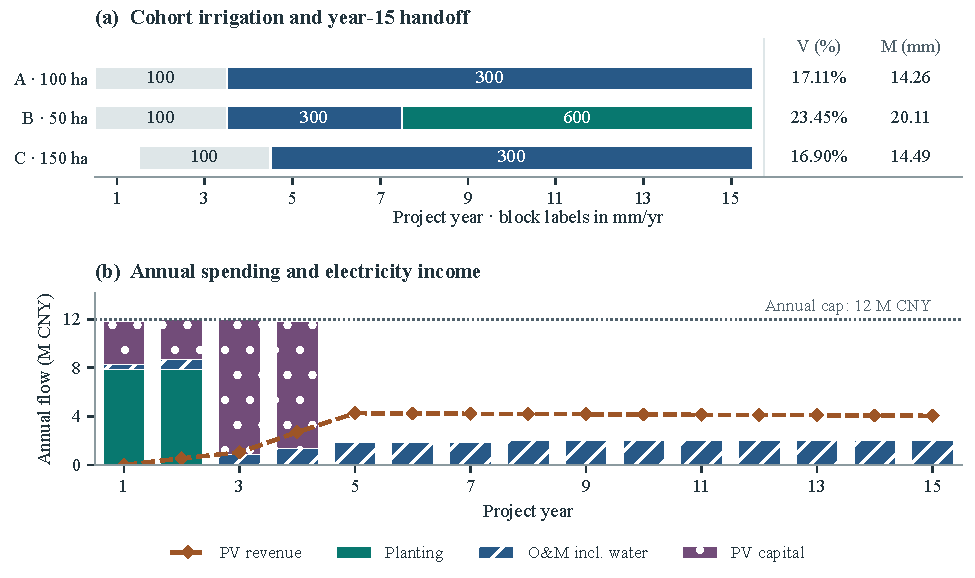
\includegraphics[width=\linewidth]{../Figures/Paper2026_Polished/fig10_cohort_plan.pdf}
  \caption{Cohort irrigation, final states and annual cash flows at the 60\% target.}
  \label{fig:m2-plan}
\end{figure}

\begin{figure}[!htbp]
  \centering
  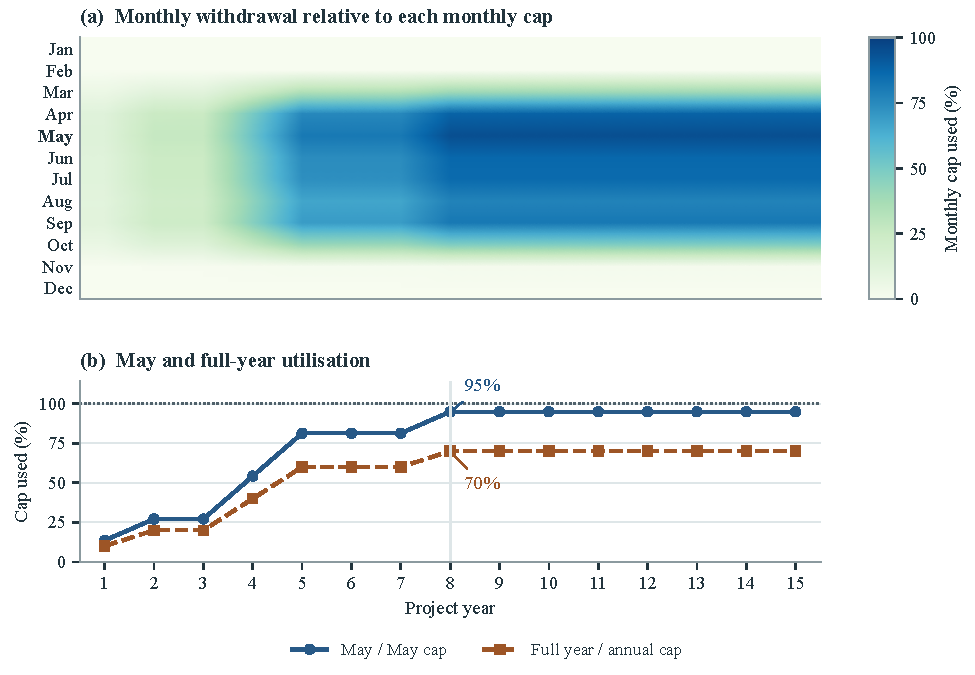
\includegraphics[width=\linewidth]{../Figures/Paper2026_Polished/fig11_water_use_smooth.pdf}
  \caption{Monthly withdrawals and the May bottleneck (interpolated shading).}
  \label{fig:m2-water}
\end{figure}

\paragraph{Balancing ecology against cost.} Up to the $60\%$ target, net present cost rises by $23\text{--}26$\,k\,CNY per added effective hectare-year across the solved targets. This increment rises to $36.7$\,k from $60\%$ to $80\%$ and $57.1$\,k from $80\%$ to $100\%$, as PV falls from $9.5$ to $5.3$\,MW and then to zero (Figure~\ref{fig:m2-tradeoff}).

For a candidate build year, the standalone tariff screen divides discounted cost by discounted generation through year~15, excluding resource opportunity costs, tax and financing. The tariff of $0.30$\,CNY/kWh clears the year-4 requirement of $0.293$ but falls short of $0.312$ in year~5. The MILP then accounts for scarce water, labour and capital.

\begin{figure}[!htbp]
  \centering
  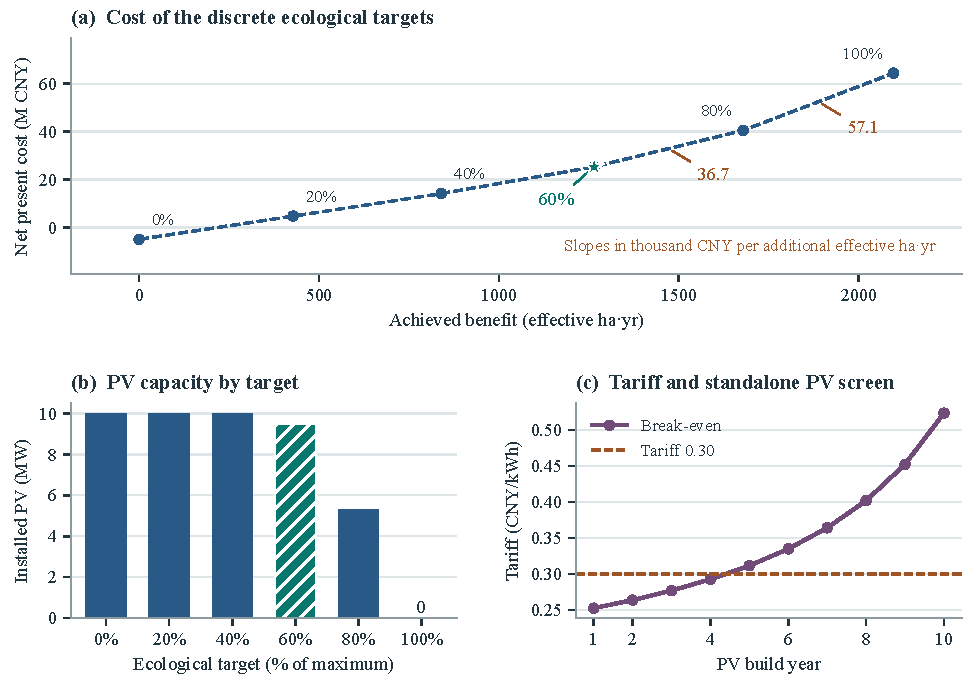
\includegraphics[width=\linewidth]{../Figures/Paper2026_Polished/fig12_tradeoff.pdf}
  \caption{Cost, ecological benefit and PV viability across six targets.}
  \label{fig:m2-tradeoff}
\end{figure}

\paragraph{Investment sensitivity.} At the same absolute ecological target, restricting the policy library to constant irrigation raises net present cost from $25.35$ to $27.04$\,M\,CNY, or about $6.6\%$ relative to the baseline. A tariff of $0.15$\,CNY/kWh or PV capex of $3{,}750$\,CNY/kW eliminates PV in the corresponding plan. Raising O\&M rates by $50\%$ trims PV to $5.6$\,MW. Halving initial cover from $2\%$ to $1\%$ raises the area required to $400$\,ha and produces the largest cost increase among the cases shown (Figure~\ref{fig:m2-investment}).

\begin{figure}[!htbp]
  \centering
  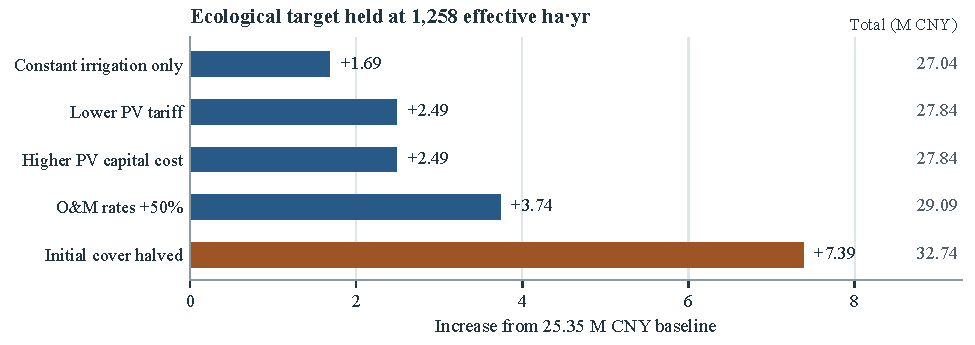
\includegraphics[width=\linewidth]{../Figures/Paper2026_Polished/fig13_investment_sensitivity.pdf}
  \caption{Cost sensitivity at a fixed ecological target.}
  \label{fig:m2-investment}
\end{figure}

\paragraph{Summary.} The conditional plan prioritizes early planting, staged irrigation and viable PV investment. May delivery capacity and seedling establishment are the main constraints to verify before adopting the plan. The completed cohorts then enter Model~3.
\FloatBarrier

% Model 3: inherited states, compound hazards, numerical check and resilience results.
\subsection{Post-Construction Resilience under Compound Disasters}\label{sec:model3}
Task~3 tests the completed belt for 50 years from Model~2's year~15 ($t=0$). Random droughts constrain canal supply, storms remove cover, and Model~1 tracks subsequent growth and recovery.

\subsubsection[Drought Rationing and Storm Damage]{Model construction}
\paragraph{Inherited stands and compound hazards.} The stress test starts from the year-15 cover, soil water and irrigation quotas of cohorts A, B and C (Figure~\ref{fig:m2-plan}a). Disasters enter through two channels \cite{EN14,EN15}. A shared yearly drought switch $D_t^{\mathrm{dr}}$ cuts rain ($\times0.40$), raises demand ($\times1.15$), shrinks canal caps ($\times0.70$) and multiplies the storm rate by $1.5$. Sandstorms, abrasion and burial are represented by a random loss of cover:
\begin{equation}\label{eq:m3-hazard}
N_t\mid D_t^{\mathrm{dr}}\sim\mathrm{Poisson}\big(\lambda_0 e^{\alpha_\lambda t}\gamma^{D_t^{\mathrm{dr}}}\big),\qquad
R_t=\prod_{q=1}^{N_t}(1-U_{t,q}),\quad U_{t,q}\sim\mathrm{U}(0.10,0.50).
\end{equation}
Climate drift slowly raises wind ($e^{\alpha_u t}$, acting through Model~1's $\mathrm{ET}_0$) and lowers rain ($e^{\alpha_R t}$).

\paragraph{One year of the belt.} Canal water is rationed month by month (PV washing first, the rest shared in proportion to requests), the unchanged Model~1 map $\Phi$ grows each cohort, and the storm retention is applied at year end:
\begin{equation}\label{eq:m3-step}
(\widetilde V_{j,t+1},\,M_{j,t+1})=\Phi\big(V_{j,t},M_{j,t};I_{j,t,m}\big),\qquad V_{j,t+1}=R_t\,\widetilde V_{j,t+1}.
\end{equation}
A warning occurs when half the belt is simultaneously below $0.30K$ ($11.4\%$ cover). Resistance is the restricted mean time to first warning, $\mathrm{RMST}(50)=\mathbb E[\min(\tau_{\mathrm{proj}},50)]$, and recovery is the difference between ever-crossed and currently low area. The physical state $(V,M)$ continues after a warning, allowing regrowth.

\subsubsection[Monte Carlo Stress Tests and Markov Verification]{Solution approach}
We simulate $6{,}000$ paths over 50 years for each reference case and $3{,}000$ per sensitivity case. Baseline storm rate is $\lambda_0=0.25$/yr, drought probability is $0.12+0.002t$, and annual wind, rain and storm-rate trends are $+0.5\%$, $-0.5\%$ and $+1\%$. These are declared stress scenarios, not calibrated forecasts. Tests vary storm rate and loss on a $3\times3$ grid, remove drought, its storm multiplier or climate drift, and compare warning levels $0.20K$ and $0.40K$.

An independent stationary Markov calculation groups stands by cover and stored water. Figure~\ref{fig:m3-check} compares its first-warning probabilities with Monte Carlo 95\% intervals at years 10, 30 and 50. Recovery and project-level outcomes come from the continuing non-stationary simulation.

\begin{figure}[!htbp]
  \centering
  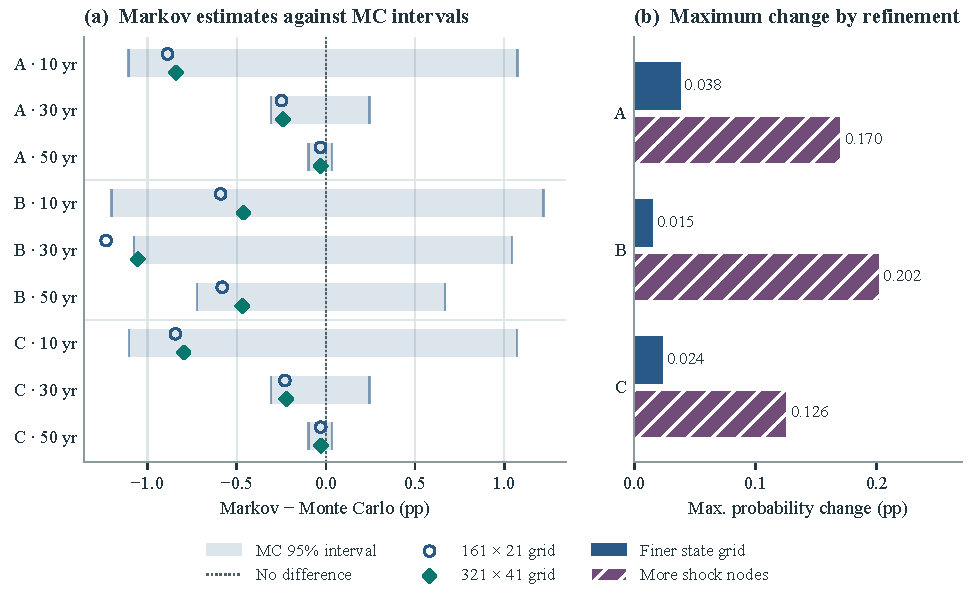
\includegraphics[width=\linewidth]{../Figures/Paper2026_Polished/fig14_markov_validation.pdf}
  \caption{Stationary Markov validation and refinement sensitivity.}
  \label{fig:m3-check}
\end{figure}

\subsubsection[Warning Risk, Vegetation Recovery, and Water Limits]{Results}
\paragraph{Early warnings and partial recovery.} In the baseline simulation, $77.5\%$ of paths trigger a belt warning by year~10, and all $6{,}000$ paths do so by year~50. The 50-year restricted mean time to first warning is $7.1$\,yr for the belt and $16.1$\,yr for core strip B (Figure~\ref{fig:m3-res}a). By year~50, almost all $300$\,ha has crossed the threshold at some point. About $99$\,ha has returned above the threshold and $200$\,ha is still below it (Figure~\ref{fig:m3-res}b). Cumulative benefit is $4{,}762\text{ effective ha}\cdot\text{yr}$, or $65.5\%$ of the climate-drift-only case (Figure~\ref{fig:m3-res}d).

\begin{figure}[!htbp]
  \centering
  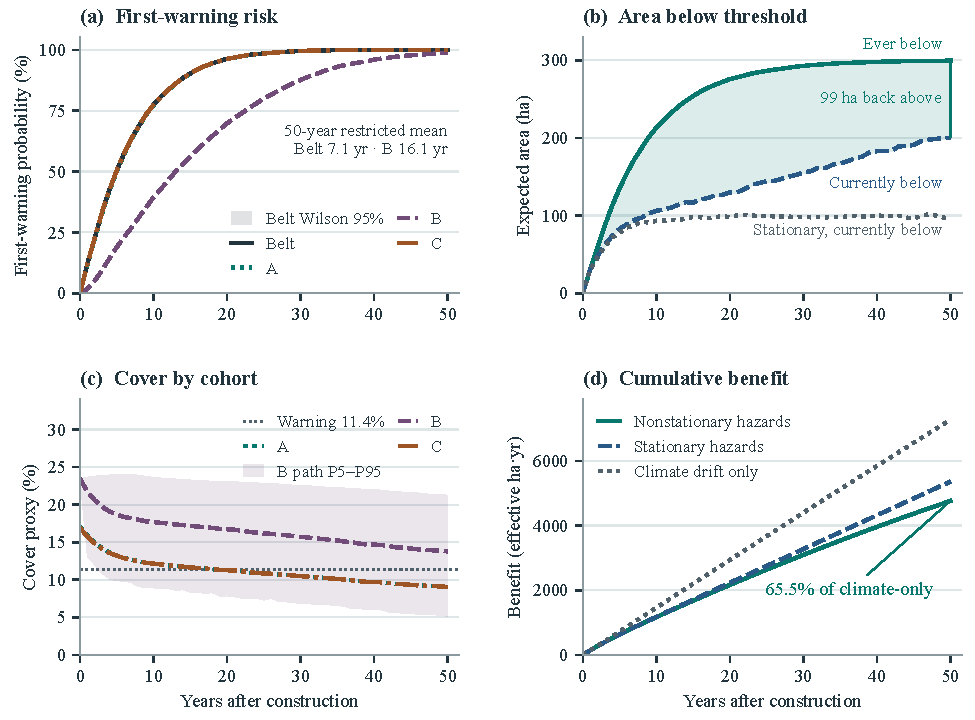
\includegraphics[width=\linewidth]{../Figures/Paper2026_Polished/fig15_resilience.pdf}
  \caption{First-warning risk, recovery and cumulative ecological benefit.}
  \label{fig:m3-res}
\end{figure}

\paragraph{Risk drivers and verification.} $\mathrm{RMST}(50)$ ranges from $41.8$\,yr for rare, mild storms to $2.8$\,yr for frequent, severe storms (Figure~\ref{fig:m3-sens}a). Requesting $20\%$ more water raises the baseline value from $7.1$ to $8.1$\,yr (panel b). In May of the first post-construction drought year, both plans receive the same $126{,}000$\,m$^3$ of ecological water at the delivery limit (panel c, rounded). That is about $26\%$ below normal May delivery under the baseline request. In the stationary check, all nine fine-grid estimates lie within the Monte Carlo $95\%$ intervals (Figure~\ref{fig:m3-check}). Refining the state grid and storm quadrature changes probabilities by at most $0.04$ and $0.20$ percentage points, respectively.

\paragraph{Summary.} Some stands regain cover after a warning. In the tested scenarios, the dry-season capacity to deliver water limits the value of raising the annual request.

In Figure~\ref{fig:m3-res}, bands show 95\% Wilson intervals for belt risk and 5th--95th path percentiles for cohort B cover. In Figure~\ref{fig:m3-sens}, the 30\% mean-loss grid column uses $[0.15,0.45]$ for loss per storm, versus $[0.10,0.50]$ in the baseline.

% Finish the preceding floats before placing this exhibit and the overall assessment.
\clearpage
\begin{figure}[H]
  \centering
  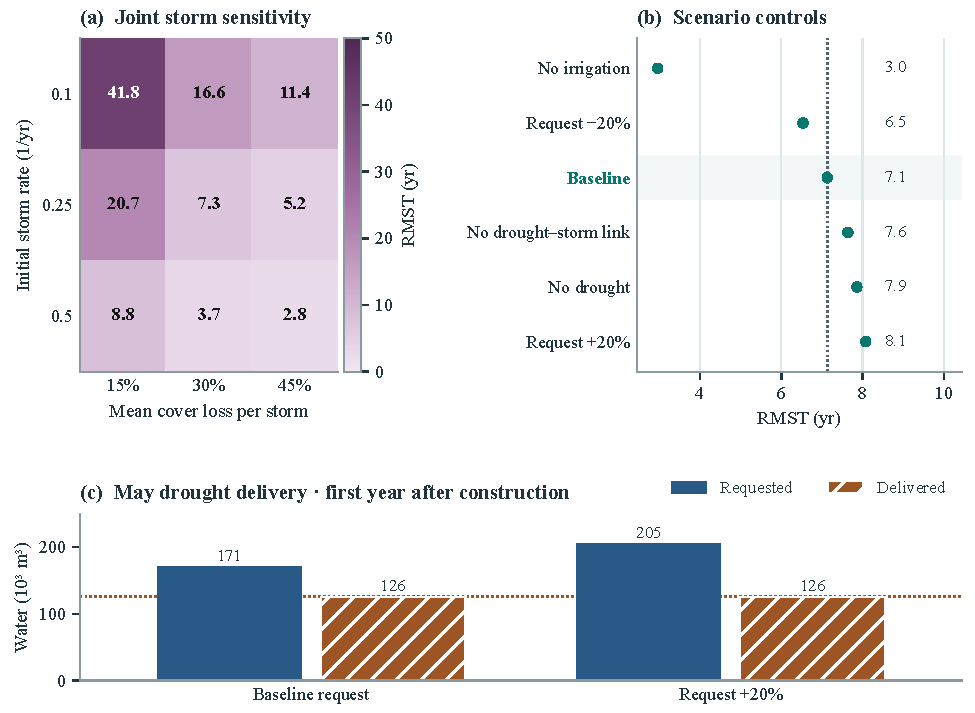
\includegraphics[width=\linewidth]{../Figures/Paper2026_Polished/fig16_storm_and_delivery.pdf}
  \caption{Storm sensitivity and May irrigation delivery under drought.}
  \label{fig:m3-sens}
\end{figure}


\Needspace{7\baselineskip}
\section{Strengths and Weaknesses}
\paragraph{Strengths.} Model~3 starts from the year-15 cover and soil water of each Model~2 cohort, preserving its irrigation history. Daily water accounting and monthly delivery caps expose limits that annual totals can hide. The MILP plan is independently replayed for water and cash closure. Stationary Markov checks support numerical consistency, while the continuing Monte Carlo paths track regrowth after a warning.

\paragraph{Weaknesses.} One-step hold-out RMSE is higher than persistence overall. Root-zone parameters, local costs, delivery limits and tariffs lack section-scale measurements. The optimisation searches 18 irrigation schedules and its selected plan depends on the declared inputs. Disaster rates, losses and warning thresholds are stress-test assumptions. Local field measurements and a damage catalogue would help assess whether these scenarios span the actual risks.

% Task 4: an unnumbered, one-page letter to the responsible officials.
\clearpage
\begingroup\small
\setlength{\parindent}{0pt}
\setlength{\parskip}{5pt}
\phantomsection
\addcontentsline{toc}{section}{Policy Letter: Holding the Taklamakan Green Belt}
\label{sec:brief}
{\large\bfseries Holding the Taklamakan Green Belt: A Practical Operating Plan\par}
\vspace{3pt}
\textbf{To:} County officials responsible for forestry, water resources, and project finance\par
Our study of the Yutian--Minfeng section links a 15-year construction and operating plan with a further 50-year disaster stress test. The baseline schedule below offers a practical starting point, conditional on reliable water deliveries, funded maintenance, and viable electricity sales.\par
\textbf{Secure water before expanding.} Confirm monthly deliveries before approving new planting. Baseline May demand reaches 95\% of monthly delivery capacity, making spring supply the immediate bottleneck. Service pumps and drip lines before May; postpone expansion if existing stands lack water and publish drought allocation rules.\par
\textbf{Make maintenance accountable.} Assign each block a supervisor and check survival after planting and the first summer. Increase irrigation as stands mature, check soil moisture before changing deliveries, and correct irrigation faults or burial damage before replanting.\par
\textbf{Structure financing and ring-fence PV revenue.} The baseline requires about CNY 44.3 million in planting and PV capital during years 1--4. During years 5--15, modelled annual PV income of CNY 4.1--4.3 million exceeds annual upkeep and water costs of CNY 1.8--2.0 million. We recommend public funding for planting and essential water infrastructure, with the operator responsible for upkeep. Earmark viable PV revenue for maintenance, equipment replacement, and a disaster reserve. Itemise annual costs, review spending quarterly, and secure funding gaps before expansion; these revenues depend on electricity prices and operating conditions.\par
\textbf{Protect communities and report results.} Prioritise vulnerable sections near roads, settlements, and farmland, and include local workers in maintenance contracts. Coordinate irrigation with household and agricultural needs. Publish vegetation condition, water deliveries, spending, and unfinished repairs annually, with a contact for public reports.\par
The implementation schedule below summarises concrete actions and lead responsibilities across phases:


\vspace{2pt}
\begingroup\footnotesize
\setlength{\tabcolsep}{4pt}\renewcommand{\arraystretch}{1.18}
\begin{tabularx}{\linewidth}{@{}>{\raggedright\arraybackslash}p{0.16\linewidth} >{\raggedright\arraybackslash}X >{\raggedright\arraybackslash}p{0.23\linewidth}@{}}
\toprule
\textbf{When} & \textbf{Practical action} & \textbf{Lead responsibility} \\
\midrule
Years 1--2 & Plant 3 square kilometres of shelterbelt if May water deliveries can cover both existing and new stands and upkeep is funded. Otherwise, defer expansion and prioritise existing stands. & Water authority and planting contractor \\
Years 1--4 & Install up to 9.5 MW of PV if grid access and budget are secured and the tariff covers costs at the quoted installation price. If PV fails to break even, use the PV-free plan and budget for upkeep. & Project operator and finance department \\
Years 5--15 & Use earmarked operating income or dedicated upkeep funding. Inspect irrigation before May and audit spending quarterly. & Operator and irrigation team \\
Year 16 onward & Continue monitoring and funded upkeep; inspect after droughts or storms and repair recoverable stands. & Monitoring and maintenance teams \\
\bottomrule
\end{tabularx}
\endgroup\par
\textbf{Expected benefits.} Sustained care can maintain shelter near roads, settlements, and farmland while supporting recurring local maintenance work. Over 50 years, the irrigated belt exposed to droughts and storms retains 65.5\% of the benefit it provides under the same long-term climate trends alone.\par
\vspace{2pt}
Yours sincerely,\\
\textit{The Modelling Team}
\par\endgroup
\clearpage


\clearpage
\begingroup
\renewcommand*{\bibfont}{\small}
\setlength{\bibitemsep}{2pt}
\setlength{\bibparsep}{0pt}
\setlength{\emergencystretch}{3em}
\printbibliography[heading=bibintoc,title={References}]
\endgroup

\end{document}
